\documentclass[letterpaper,10pt]{article}

%\setlength{\parindent}{0in}
%\usepackage{fullpage} 
\usepackage{amsmath}
\usepackage{amssymb}
\usepackage{enumerate}
\usepackage{graphicx}
\usepackage{color}
\usepackage[table]{xcolor}
\usepackage{dcolumn}
\oddsidemargin 0.0in
\textwidth 6.5in
\newcolumntype{.}{D{.}{.}{-1}}
\newcommand*{\myalign}[2]{\multicolumn{1}{#1}{#2}}

%Project Assignment 2 Test and Evaluation is due 2/17/12. It is a team event. 
%Please see the Project area in Sakai for more guidance.
%Using the test results of a field test of the concept prototype IED robot variants:
%a) Provide a physical description of the system that was tested. You should 
%complete the QFD1 QFD2 and QFD3 analysis in order to determine the 
%physical forms.
%b) Provide a summary description of the Limited Objective Exercise (LOE) test
%that was conducted.
%c) Using the test results of a field test of the concept prototype IDE robot 
%variants (A, B, and C), assess the performance versus the LOE test results used 
%for OMOE determination.  Use box plots, t-tests, and ANOVA, as appropriate, 
%to compare the test results of the prototypes.  Summarize and present the 
%results of your analysis.
%Remember to complete your RPG Role Evaluation on the Discussion Board 
%also!

\title{Project 2 \\ \Large Team CLEAR \\ \normalsize (\textcolor{red}{C}onvoy \textcolor{red}{L}evel \textcolor{red}{E}xplosive \textcolor{red}{A}mmunition \textcolor{red}{R}emoval)}
\author{Christian Aall: Testing \& Evaluation \\ 
	Steve Mazza: Team Lead \\ 
	Michael Oexmann: Analyst \\ 
	Elizabeth Swisher: Lead Systems Engineer}
	
\date{February 17, 2012}

\begin{document}
\maketitle
\tableofcontents
\listoftables
\listoffigures

\vspace{2em}
In order to successfully achieve the goal of providing area specific, detection and clearance of improvised explosive devices (IEDs) while meeting stakeholder requirements, proper testing, evaluation and analysis must occur. Testing is a continuous process that should occur throughout the system's lifecycle.  There are two reasons for test and evaluation: verifying specifications/requirements and managing risk. To date, three conceptual system prototypes for the Simulated Micro Expeditionary Transforming Air Land-Vehicle (SMETAL-V) have been built and tested. This report provides a description of the tested systems, quality function deployment (QFD) diagrams based off stakeholder preferences, an outline of the conducted Limited Objective Exercise test, and a thorough summary of test results, evaluation and analysis.

\section{System Description}
Using Quality Function Deployment (QFD) diagrams we move our understanding from Customer Requirements to a physical description of the system.  Since we have requirements from two theaters of operation, Afghanistan and Iraq, we began by creating two versions of the QFD 1, mapping Customer Requirements to Design Characteristics (see Figures \ref{figQFD1a} and \ref{figQFD1b} on pages \pageref{figQFD1a} and \pageref{figQFD1b}, respectively).  We then take the Design Characteristics and map those to Functions in the QFD 2 diagrams (see Figures \ref{figQFD2a} and \ref{figQFD2b} on pages \pageref{figQFD2a} and \pageref{figQFD2b}, respectively).  Lastly we map Functions to physical Forms in the QFD 3 diagrams s (see Figures \ref{figQFD3a} and \ref{figQFD3b} on pages \pageref{figQFD3a} and \pageref{figQFD3b}, respectively).

%TODO:

We notice that there is an extremely high correlation among the Forms derived from both theaters in QFD 3.  This gives us a high degree of confidence that we can meet customer expectations in both theaters based on our gathered requirements and system drivers.

The following Forms emerge from both sets of Customer Requirements.
\subsection{IED Sensor}
The Improvised Explosive Device (IED) Sensor performs the critical task of locating and identifying an IED within the operational range of the sensor.  IED sensors are developed by the Army and continually improved and so this is an excellent opportunity for Systems Engineers to define on interface (or control point) through which the IED sensor will communicate its findings to the rest of the SMETAL-V system.  In this way, new sensor technology can be developed, adopted, and integrated into the current generation product with a minimum of re-work.
\subsection{Chassis}
The chassis serves as the basis of of the SMETAL-V platform and is the fixture onto which all other parts are fixed.  Reducing chassis weight is key to maintaining overall weight goals, balanced off against the necessity to provide a robust and reliable product.  Carefully choosing material (e.g., polycarbonite, carbon fiber, aluminum) will help engineers meet critical design goals.
\subsection{Drive Train}
The drive train provides locomotion to the SMETAL-V system and ultimately determines the type of terrain that the platform can traverse as well as the speed with which it can do so.  Electric motors develop full torque at all speeds, are efficient, and inexpensive to use over the lifecycle of the product.  They are also natural to control from the NXT Brick.  Tracked vehicles are somewhat more expensive but provide more precise maneuverability and the ability to climb steeper inclinations.
\subsection{Onboard Communications}
Onboard communications provide a path for the two-way flow of data between the operator and the SMETAL-V system and between the SMETAL-V system and the point of data collection in the event that these are not the same.  Methods of communication include radio, Bluetooth, WiFi, Xbee, and others.  Each protocol has strengths and weaknesses that affect range, jamming, duplex, error correction, encryption, and reliability, among others.  Communications protocols should be carefully evaluated for DoD compliance and suitability for use in a tactical environment.  Also, the need for integration with programs of record might dictate the method of communication.
\subsection{Weight Margin}
Meeting weight goals is often difficult and frequently relies on advances in material science in conjunction with sound engineering judgement.  Tradeoffs most often include functionality, range, size, speed, cost, and strength (durability), but may include other factors as well.  
\subsection{Fuel Capacity}
Fuel capacity is directly proportional to range and inversely proportional to weight.  Inasmuch it is a relatively easy metric to trade off.  Determining the type of fuel for the SMETAL-V platform will provide us with valid ranges of range and weight (as well as cost).  Assuming that the final fuel product will be to provide a regulated electric source for the system, obvious choices include Nickel-Cadnium (NiCad), Nickle-Metal Hydride (NiMH), and rechargeable Alkaline.  More expensive choices include photo-voltaic solar array and fuel cell technology.  Target system cost and concept of operations should dictate the most reasonable choice.
\subsection{Ground Clearance}
Ground clearance trades off mobility for stability.  Although there are mechanisms to provide relatively high ground clearance while maintaining a relatively low center of gravity, the implementation of these tends to increase the engineering effort, cost, and reduces payload capacity.
\subsection{Operational Range}
Operational range is both a component of fuel capacity and the specified reliable range of the onboard communications.  Choices affecting this are highly likely to directly affect cost.
\subsection{NXT Brick$\textsuperscript{\textregistered}$}
Built by Lego$\textsuperscript{\textregistered}$, the NXT Brick$\textsuperscript{\textregistered}$ is an inexpensive, readily available programable microcontroller that combines standardized interfaces with an easy-to-program core.  Programming is extensible by third parties and has been opened up to leverage the power and existing base of the C programming language.  The NXT Brick$\textsuperscript{\textregistered}$ will act as the control point between the operator and the SMETAL-V platform, allowing the operator full control of the vehicle's capabilities.

\section{Limited Objective Exercise}
The SMETAL-V Limited Objective Exercise (LOE) was used to test the various alternatives against a standard test set to gage the progress of the prototypes. The SMETAL-V program has had four respondents to the advanced development prototype competition, three of which developed working robots that were able to complete the LOE. To remove bias, each of the three variants competing in the LOE were identified by the labels $A$, $B$, and $C$ respectively. A contractor performed the LOE with the aid of PEO-IED and results were certified by government T\&E personnel.

The following nine steps summarize the procedure used for each test run:
\begin{enumerate}
	\item Determine the size of the SMETAL-V Storage Container.
	\item Place the SMETAL-V in the deployed state with batteries removed and SMETAL-V Programming Unit off.
	\item Place the SMETAL-V into the ready state and determine Deployed-to-Ready Time.
	\item Drop the SMETAL-V onto the DRM start position and verify Vehicle Drop Height threshold.
	\item Carry out the DRM and measure DRM Elapsed Time. Then place the SMETAL-V in the ready state.
	\item Carry out a battery replacement with new batteries to determine Refueling Time.
	\item Carry out the DRM a second time and measure DRM Elapsed Time. Then place the SMETAL-V in the ready state. 
	\item Weigh the SMETAL-V to determine Vehicle Weight using a suitable postage or other scale.
	\item Place the SMETAL-V into the deployed state, collect and organize the recorded data, and terminate the LOE.
\end{enumerate}

Each prototype conducted twenty test runs. Table \ref{tblLOE} on page \pageref{tblLOE} summarizes the average test results over the twenty trails for each prototype against KPPs.

\begin{table}[h!tdp]
\begin{center}
\begin{tabular}{lcccccc}
\hline
& & & & \multicolumn{3}{c}{\textbf{Prototype}} \\
& \myalign{c}{\textbf{Threshold}} & \myalign{c}{\textbf{Goal}} & \myalign{c}{\textbf{Units}} & \myalign{c}{\textbf{A}} & \myalign{c}{\textbf{B}} & \myalign{c}{\textbf{C}} \\
\hline\hline
Mission Reliability & 0.9 & 0.95 & & \cellcolor{yellow}0.92 & \cellcolor{yellow}0.94 & \cellcolor{yellow}0.94 \\
Operational Availability & 0.8 & 0.9 & & \cellcolor{green}0.90 & \cellcolor{yellow}0.88 & \cellcolor{green}0.92 \\
Vehicle Weight & 18 & 14 & ounces & \cellcolor{yellow}16 & \cellcolor{green}14 & \cellcolor{yellow}18 \\
Vehicle Drop Height & 1 & 3 & inches & \cellcolor{green}3 & \cellcolor{yellow}1 & \cellcolor{green}3 \\
Refueling Time & 60 & 30 & seconds & \cellcolor{yellow}48.36 & \cellcolor{yellow}51.70 & \cellcolor{yellow}39.11 \\
DRM Elapsed Time & 5 & 3 & minutes & \cellcolor{yellow}4.22 & \cellcolor{yellow}3.69 & \cellcolor{yellow}4.65 \\
Deployed-to-Ready Time & 10 & 5 & minutes & \cellcolor{yellow}7.07 & \cellcolor{yellow}8.06 & \cellcolor{yellow}6.51 \\
SMETAL-V Storage Container & 216 & 120 & in$^{3}$ & \cellcolor{yellow}188 & \cellcolor{yellow}200 & \cellcolor{yellow}204 \\
Operational Team Size & 2 & 1 & persons & \cellcolor{green}1 & \cellcolor{yellow}2 & \cellcolor{green}1 \\
\hline
\multicolumn{2}{c}{\cellcolor{green}met goal} & \multicolumn{5}{c}{\cellcolor{yellow}met threshold but not goal} \\
\end{tabular}
\end{center}
\caption{Limited objective exercise test results}
\label{tblLOE}
\end{table}

Although all of the prototypes met the thresholds on average, each prototype had a test run that failed to meet a given threshold on an individual test run. Prototype $A$ did not meet Refueling Time threshold in trial 20, recording a measure Refueling Time of 61.71 seconds versus the required 60 seconds. Prototype $B$ did not meet Deployed-to-Ready Time threshold in trials 4 or 17, recording measured Deployed-to-Ready Time 10.38 and 10.18 minutes versus the required 10 minutes respectively. Prototype $C$ did not meet DRM Elapsed Time threshold in trial 14, recording a DRM Elapsed Time of 5.01 minutes versus the required 5 minutes.

\section{Concept Prototype Performance}
A recommended approach for continued technology development can be provided by comparing the test results of the three conceptual prototypes (A, B, and C) to the established Overall Measures of Effectiveness (OMOEs ). In order to determine which of the three prototypes has most effectively achieved the OMOEs, test data was compiled and analyzed using Analysis of Variance (ANOVA), descriptive statistics and box plots. 

The first step of the analysis was to evaluate the test results (including Mission Reliability, Refueling Time, DRM Elapsed Time, and Deployed-to-Ready Time) calculate Operational Availability, and measure system characteristics (including Vehicle Weight, Vehicle Drop Height, Storage Container Volume, and Operational Team Size) against Key Performance Parameters (KPPs). This comparison was conducted using ANOVA. Utilizing this method of analysis allowed each system to be compared by its statistical similarity to KPPs.

The ANOVA results indicate that all three prototypes failed to show statistical similarity to KPPs � this is expected as these systems are still prototypes and require increased maturity. However, the results also indicate which of the three prototypes is the closest to meeting KPPs. Because each prototype, on average, was able to meet or exceed the threshold KPPs, the ANOVA focused on comparison to KPP goal values.

The Summary and ANOVA outputs for each prototype can be seen below in Tables \ref{tabA} - \ref{tabC} beginning on page \pageref{tabA}.

\begin{table}[h!tdp]
\begin{center}
\begin{tabular}{l....rr}
\hline
\textsc{\textbf{Summary}} & & & & & & \\
\myalign{c}{\textbf{Groups}} & \myalign{c}{\textbf{Count}} & \myalign{c}{\textbf{Sum}} & \myalign{c}{\textbf{Average}} & \myalign{c}{\textbf{Variance}} & & \\
\hline\hline
A & 9 & 269.47 & 29.94 & 3743.70 & & \\
Goal & 9 & 177.85 & 19.76 & 1503.40 & & \\
\hline
\textsc{\textbf{ANOVA}} & & & & & & \\
\myalign{c}{\textbf{Source of Variation}} & \myalign{c}{\textbf{SS}} & \myalign{c}{\textbf{df}} & \myalign{c}{\textbf{MS}} & \myalign{c}{\textbf{F}} & \myalign{c}{\textbf{P-value}} & \myalign{c}{\textbf{F crit}} \\
\hline
\hline
Between Groups & 466.40 & 1 & 466.40 & 0.18 & \cellcolor{yellow}{0.68} & 4.49 \\
Within Groups & 41976.82 & 16 & 2623.55 & & & \\
Total & 42443.21 & 17 & & & & \\
\hline
\end{tabular}
\end{center}
\caption{Results of prototype $A$ vs. goal}
\label{tabA}
\end{table}

\begin{table}[h!tdp]
\begin{center}
\begin{tabular}{l....rr}
\hline
\textsc{\textbf{Summary}} & & & & & & \\
\myalign{c}{\textbf{Groups}} & \myalign{c}{\textbf{Count}} & \myalign{c}{\textbf{Sum}} & \myalign{c}{\textbf{Average}} & \myalign{c}{\textbf{Variance}} & & \\
\hline\hline
A & 9 & 282.26 & 31.36 & 4262.67 & & \\
Goal & 9 & 177.85 & 19.76 & 1503.40 & & \\
\hline
\textsc{\textbf{ANOVA}} & & & & & & \\
\myalign{c}{\textbf{Source of Variation}} & \myalign{c}{\textbf{SS}} & \myalign{c}{\textbf{df}} & \myalign{c}{\textbf{MS}} & \myalign{c}{\textbf{F}} & \myalign{c}{\textbf{P-value}} & \myalign{c}{\textbf{F crit}} \\
\hline
\hline
Between Groups & 605.65 & 1 & 605.65 & 0.21 & \cellcolor{yellow}{0.65} & 4.49 \\
Within Groups & 46128.56 & 16 & 2883.04 & & & \\
Total & 46734.22 & 17 & & & & \\
\hline
\end{tabular}
\end{center}
\caption{Results of prototype $B$ vs. goal}
\label{tabB}
\end{table}

\begin{table}[h!tdp]
\begin{center}
\begin{tabular}{l....rr}
\hline
\textsc{\textbf{Summary}} & & & & & & \\
\myalign{c}{\textbf{Groups}} & \myalign{c}{\textbf{Count}} & \myalign{c}{\textbf{Sum}} & \myalign{c}{\textbf{Average}} & \myalign{c}{\textbf{Variance}} & & \\
\hline\hline
A & 9 & 278.13 & 30.90 & 4368.81 & & \\
Goal & 9 & 177.85 & 19.76 & 1503.40 & & \\
\hline
\textsc{\textbf{ANOVA}} & & & & & & \\
\myalign{c}{\textbf{Source of Variation}} & \myalign{c}{\textbf{SS}} & \myalign{c}{\textbf{df}} & \myalign{c}{\textbf{MS}} & \myalign{c}{\textbf{F}} & \myalign{c}{\textbf{P-value}} & \myalign{c}{\textbf{F crit}} \\
\hline
\hline
Between Groups & 558.68 & 1 & 558.68 & 0.19 & \cellcolor{yellow}{0.67} & 4.49 \\
Within Groups & 46977.65 & 16 & 2936.10 & & & \\
Total & 47536.33 & 17 & & & & \\
\hline
\end{tabular}
\end{center}
\caption{Results of prototype $C$ vs. goal}
\label{tabC}
\end{table}

Based on the results, prototype $B$ is statistically \emph{most similar} to the KPP goal values. Its associated ANOVA output indicates the lowest $p-$value when compared to prototypes $A$ and $C$.  Descriptive statistics and box plots were also used to gain additional prototype performance insights.

Box plots allow for quick visual comparisons of test data and help to verify the findings discovered through ANOVA. In order to create box plots for each of the KPPs, descriptive statistics were generated and used as input. The box plots created as a result of this analysis can be seen below in Figures \ref{figA} - \ref{figD} beginning on page \pageref{figA}.

The box plots depict the median, minimum, maximum, and inter-quartile range for a given set of data. In this regard they are especially useful as they allow for a more accurate analysis of a data set than the plot of averages alone. Based on the box plots it is evident that prototypes $B$ and $C$ are consistently the best performing and closest to the goal values for each metric. If prototype selection was solely based on a visual analysis of box plots, one would recommend variant $C$ for its strong Refueling Time and Deployed-to-Ready-Time. On the other hand, the ANOVA analysis above indicated prototype $B$ as the most statistically similar, therefore a more complete analysis of the data must be performed.

Testing of the prototypes was limited to the four metrics depicted in the box plots, however, data is available for the five remaining KPP metrics and should also be charted for visual comparison purposes.  The remaining data is charted below in Figures \ref{figE} - \ref{figI} beginning on page \pageref{figE}.

As one can infer from the charts above, $B$ is the closest to the goal values while still consistently exceeding the threshold. One must consider that the ANOVA analysis does not necessarily indicate which variant is highest performing, but simply which variant�s data set reflects highest congruency with the threshold and goal values. A variant that far exceeds both threshold and goal values will not indicate statistical similarity as seen in the $p-$value. 

\section{Summary}
Given a thorough and complete analysis of the provided data and test results, prototype $C$ has been determined to outperform prototypes $A$ and $B$ overall.

This thorough analysis of design characteristics and their relevance to customer requirements allowed for recommendations to be drawn regarding prototype variants for further consideration. The QFD analysis ensured that we effectively met Afghanistan and Iraq customer requirements, and provided for an evaluation of the level of performance provided by each design criteria vs. the respective requirements.
	
The assessment of the individual functional features of the SMETAL-V system will result in further technology trade off studies and potentially function as guideline for capability integration. Through the use of variance analysis, a report on the statistical similarity of test data means to the provided thresholds and goals was provided. It was concluded that such an assessment alone would not provide for a complete analysis of the highest performing variant, but instead only state absolute similarity between a data set and a constant value. Further analysis revealed that prototype variant $C$ was the highest performing overall, and still met all the KPP thresholds.
	
It is our recommendation that we proceed with development and further test and evaluation of prototype variant $C$. A higher level effort will be applied to improving the DRM Elapsed Time KPP values of variant $C$ to ensure that the prototype variant meets or exceeds the goal value.

\pagebreak
\appendix
\section{Quality Function Deployment Diagrams}

\begin{figure}[h!tbp]
\begin{center}
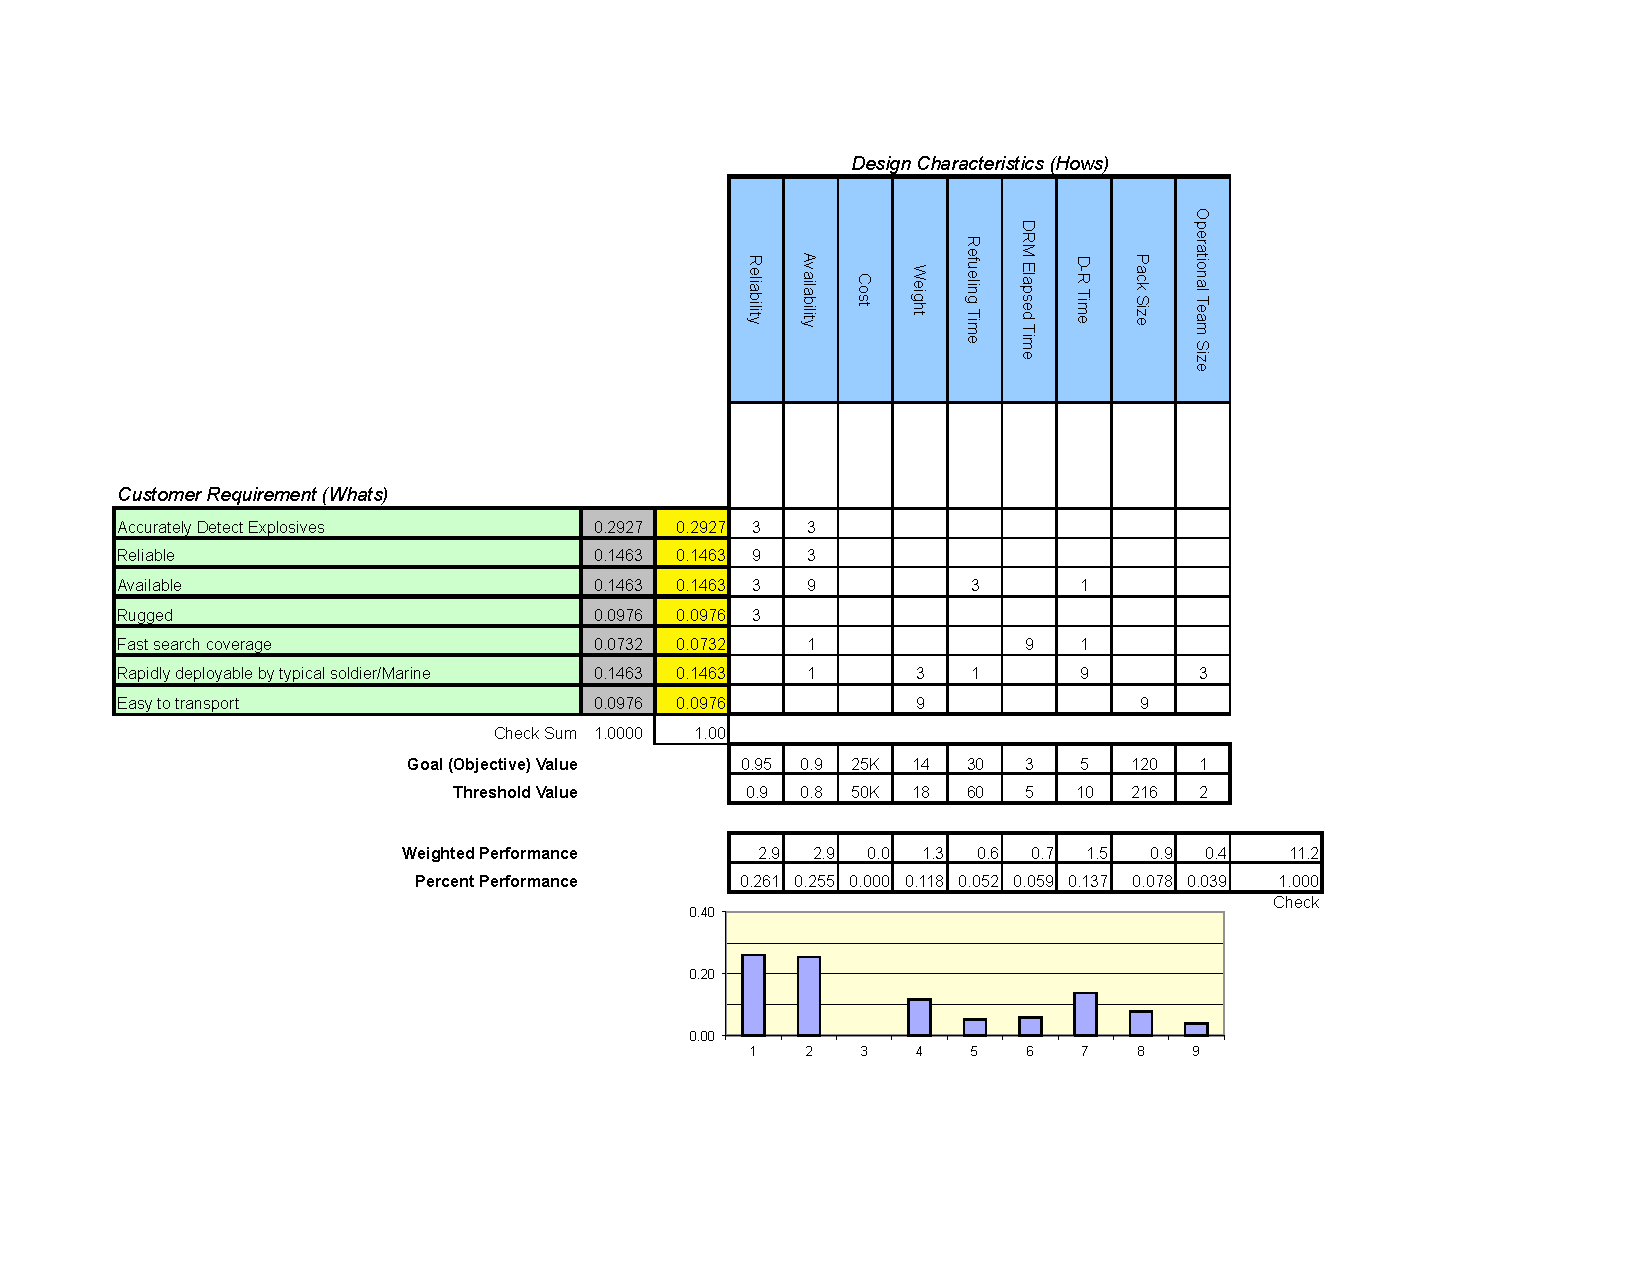
\includegraphics[scale=0.75]{QFD1a.pdf}
\caption{QFD 1 - Afghanistan}
\label{figQFD1a}
\end{center}
\end{figure}

\begin{figure}[h!tbp]
\begin{center}
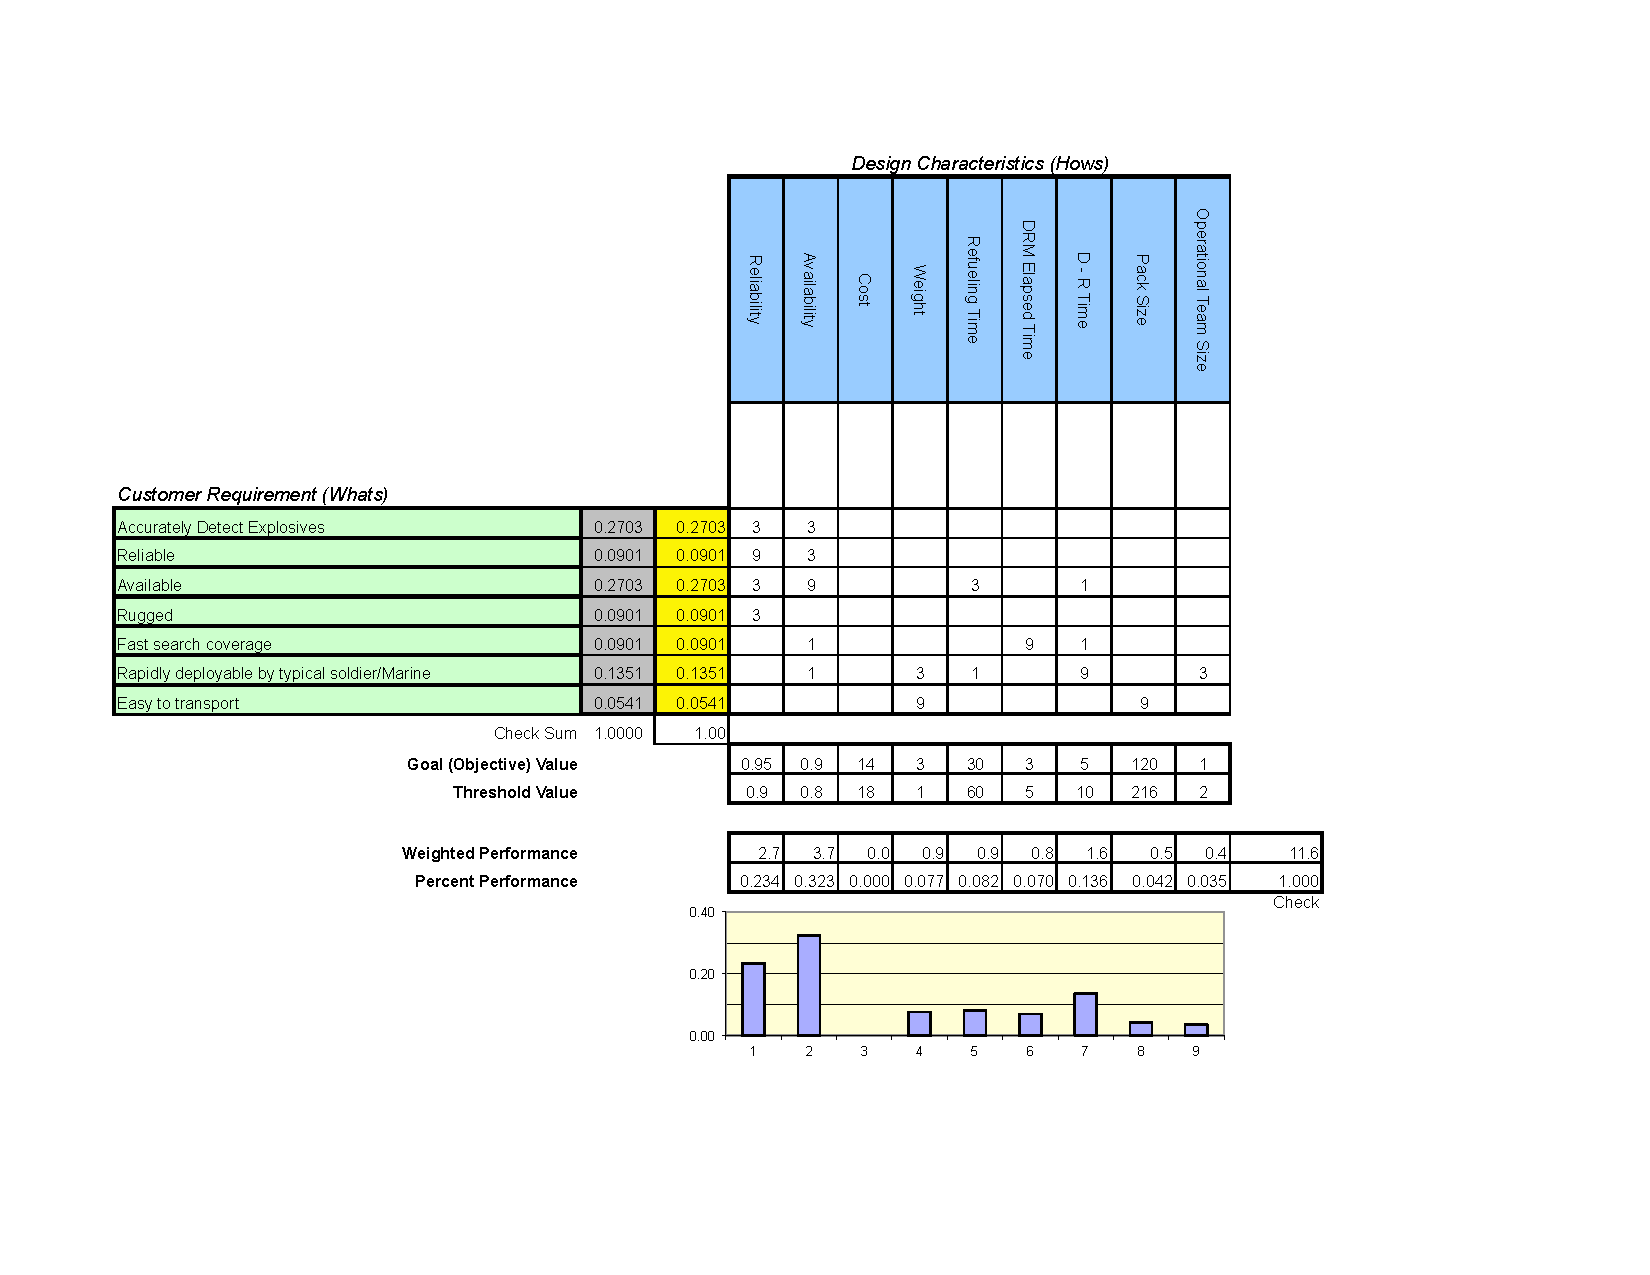
\includegraphics[scale=0.75]{QFD1b.pdf}
\caption{QFD 1 - Iraq}
\label{figQFD1b}
\end{center}
\end{figure}

\begin{figure}[h!tbp]
\begin{center}
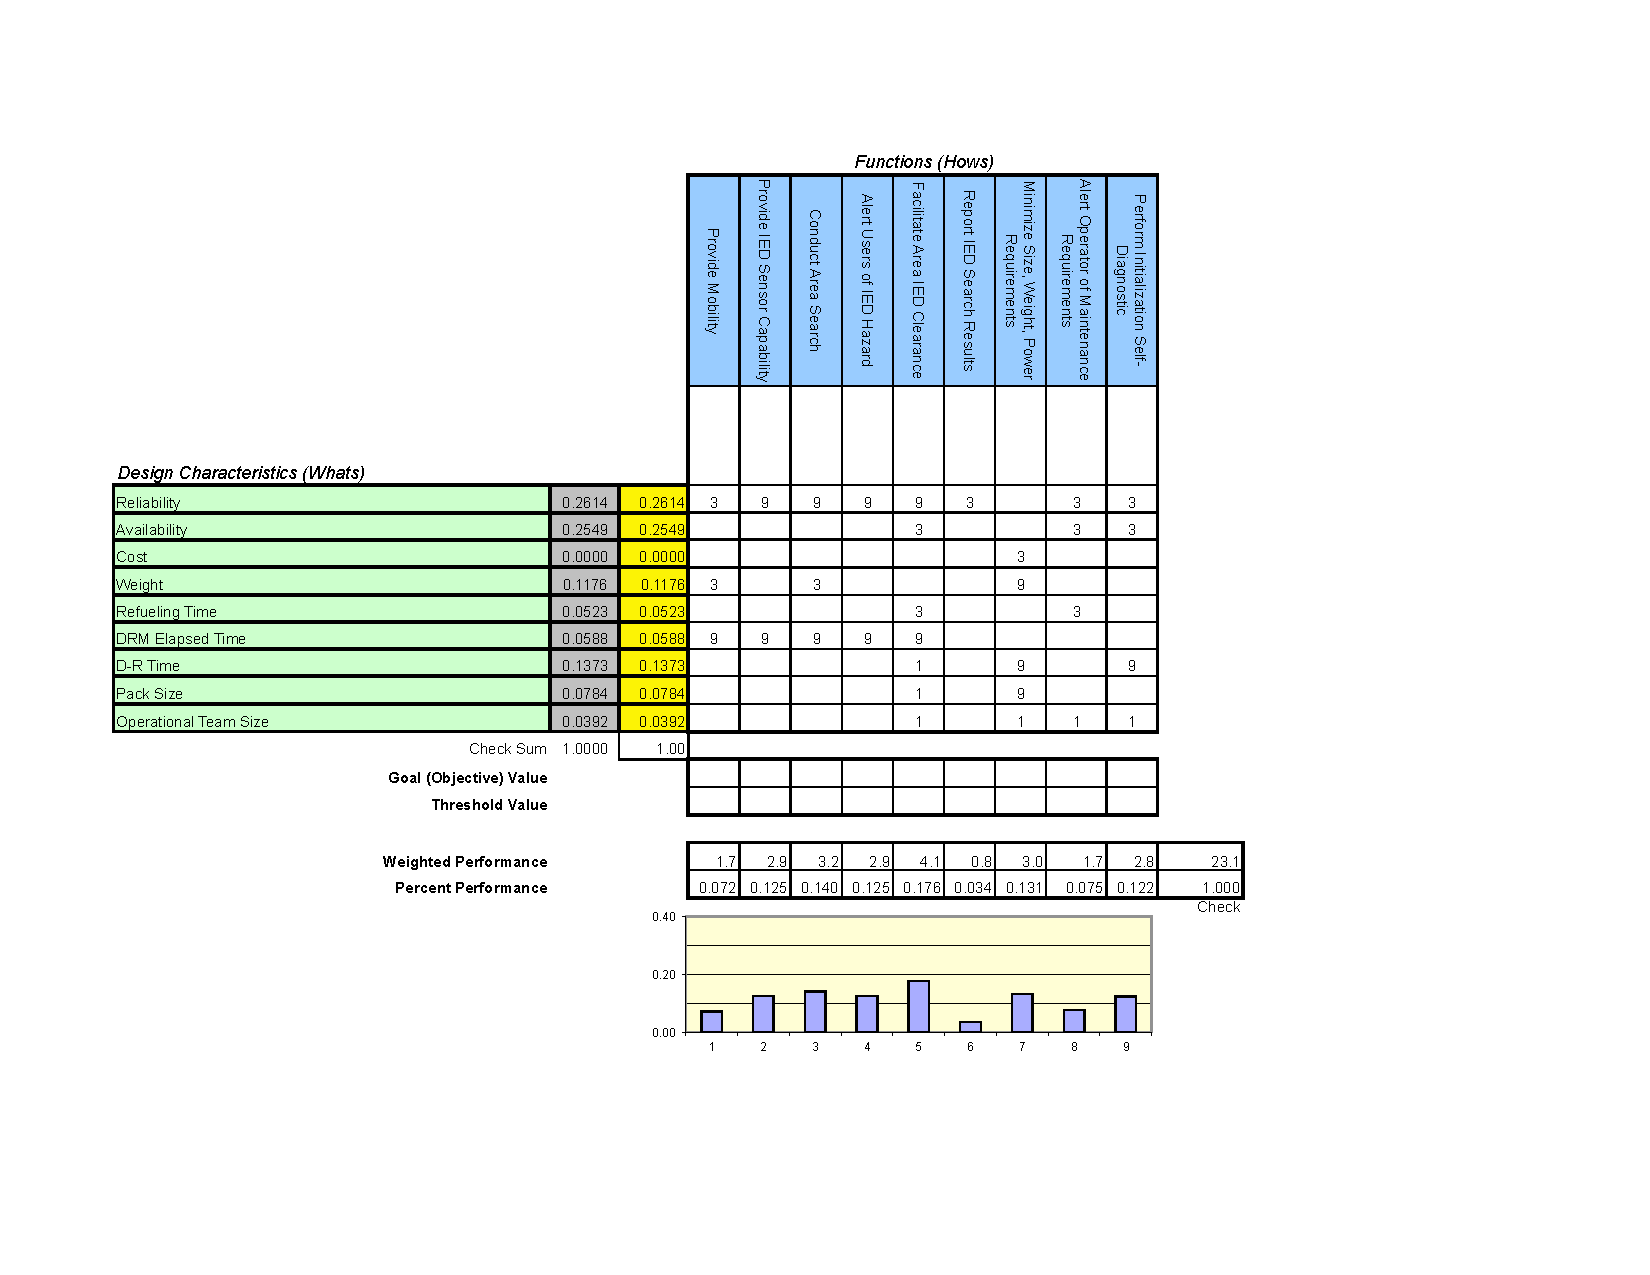
\includegraphics[scale=0.75]{QFD2a.pdf}
\caption{QFD 2 - Afghanistan}
\label{figQFD2a}
\end{center}
\end{figure}

\begin{figure}[h!tbp]
\begin{center}
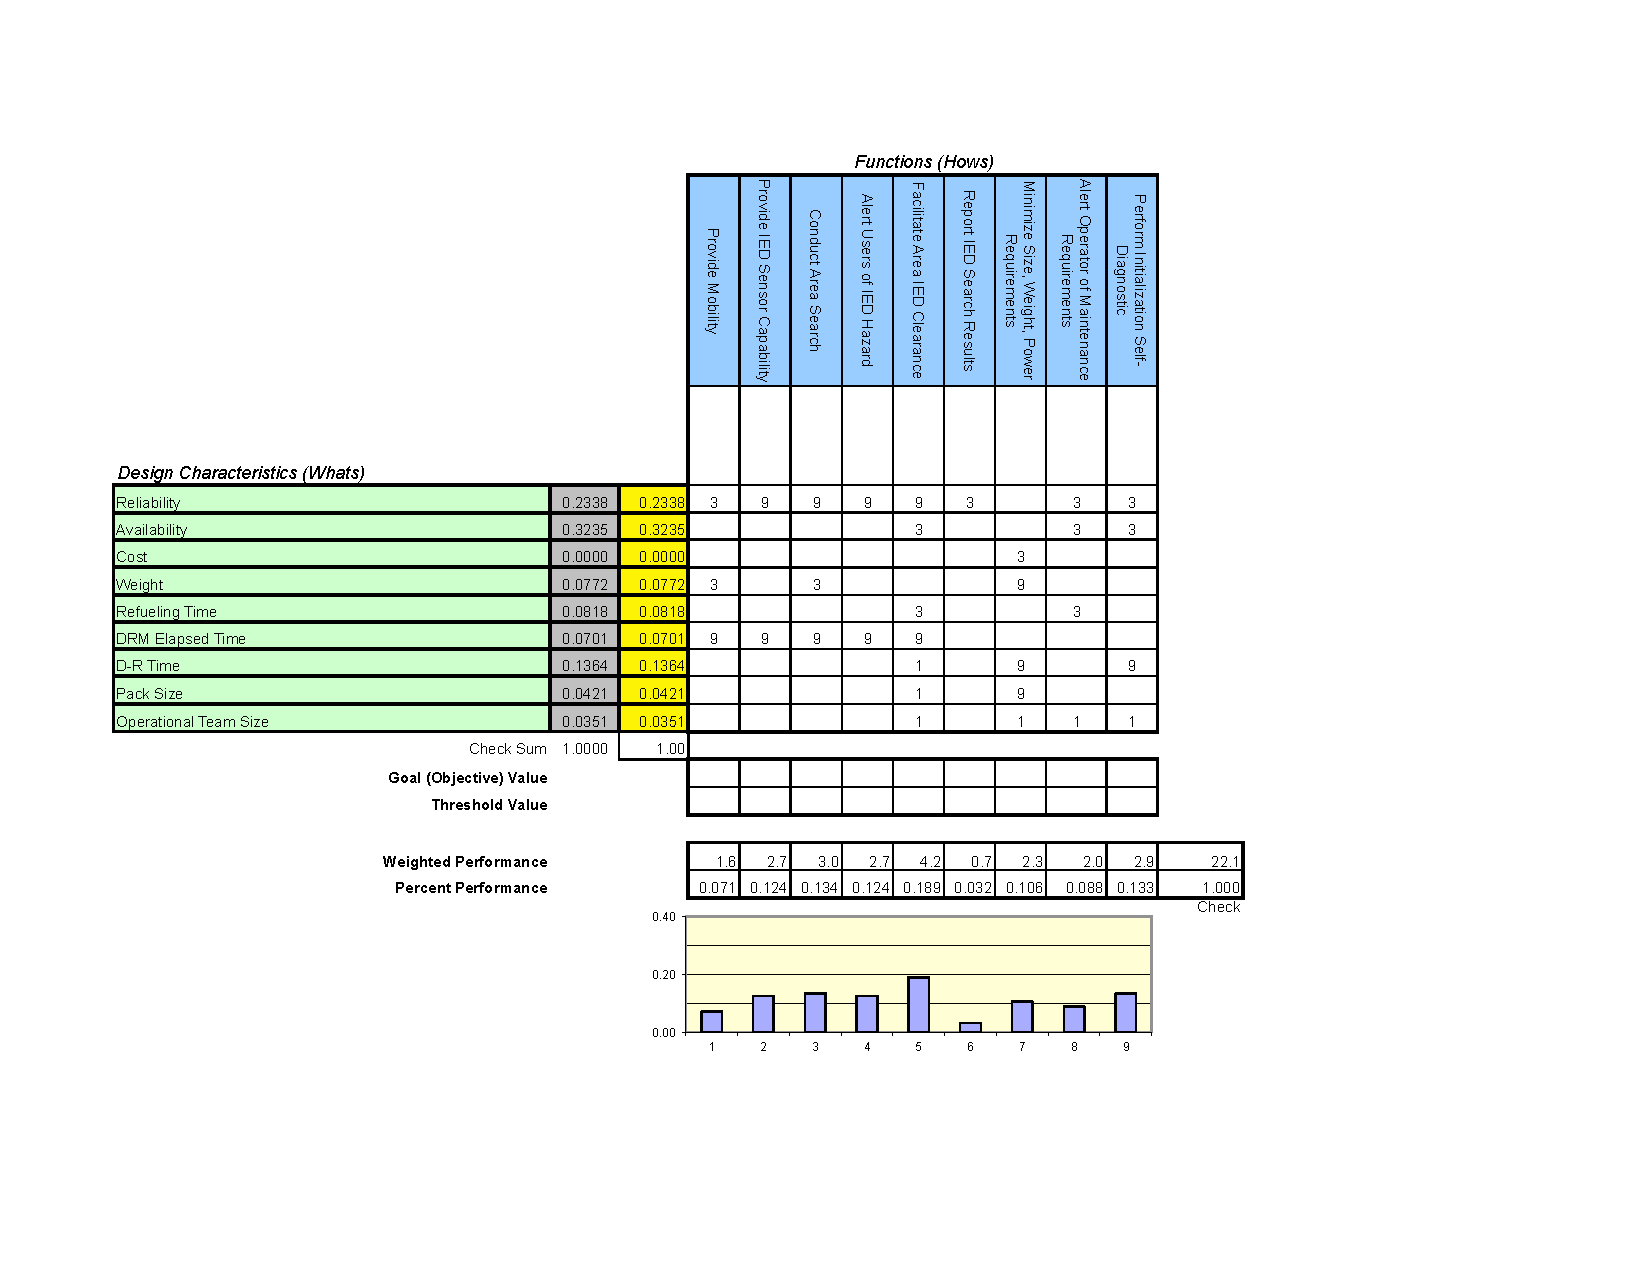
\includegraphics[scale=0.75]{QFD2b.pdf}
\caption{QFD 2 - Iraq}
\label{figQFD2b}
\end{center}
\end{figure}

\begin{figure}[h!tbp]
\begin{center}
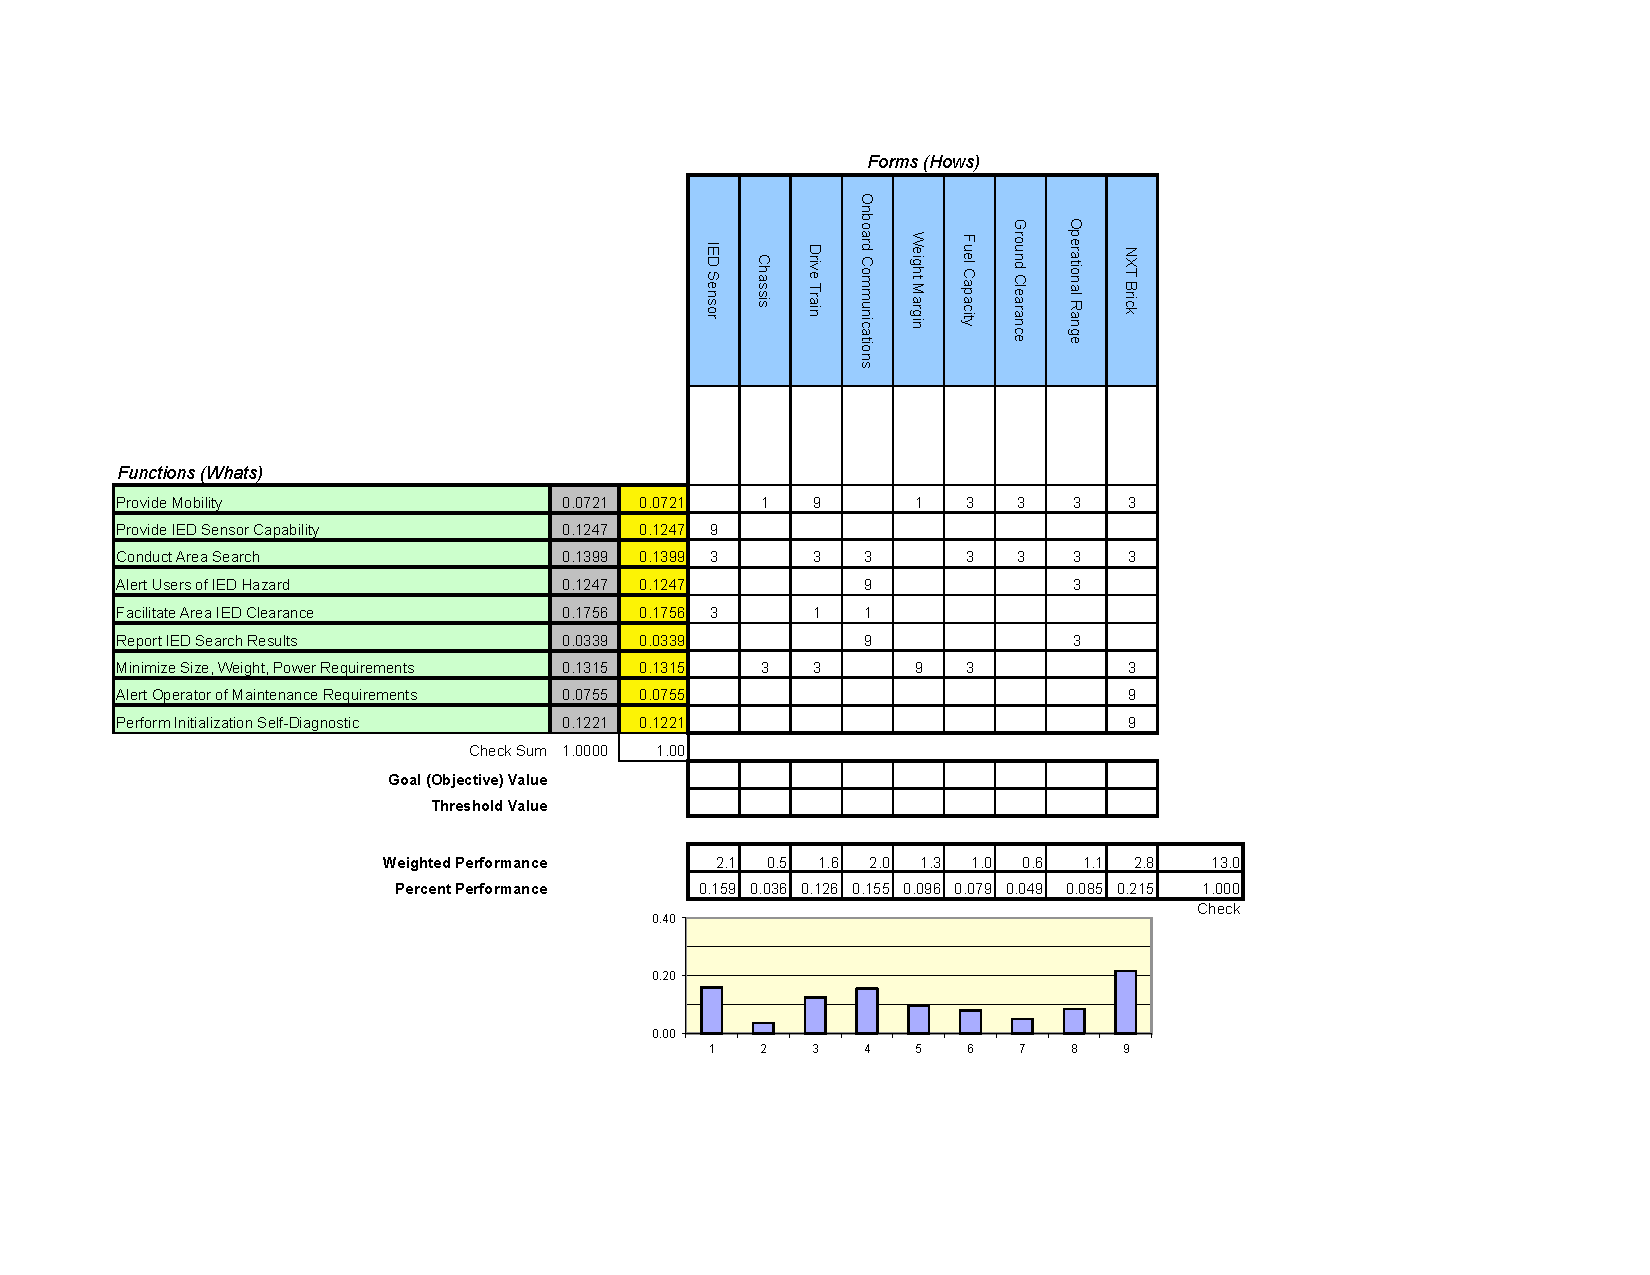
\includegraphics[scale=0.75]{QFD3a.pdf}
\caption{QFD 3 - Afghanistan}
\label{figQFD3a}
\end{center}
\end{figure}

\begin{figure}[h!tbp]
\begin{center}
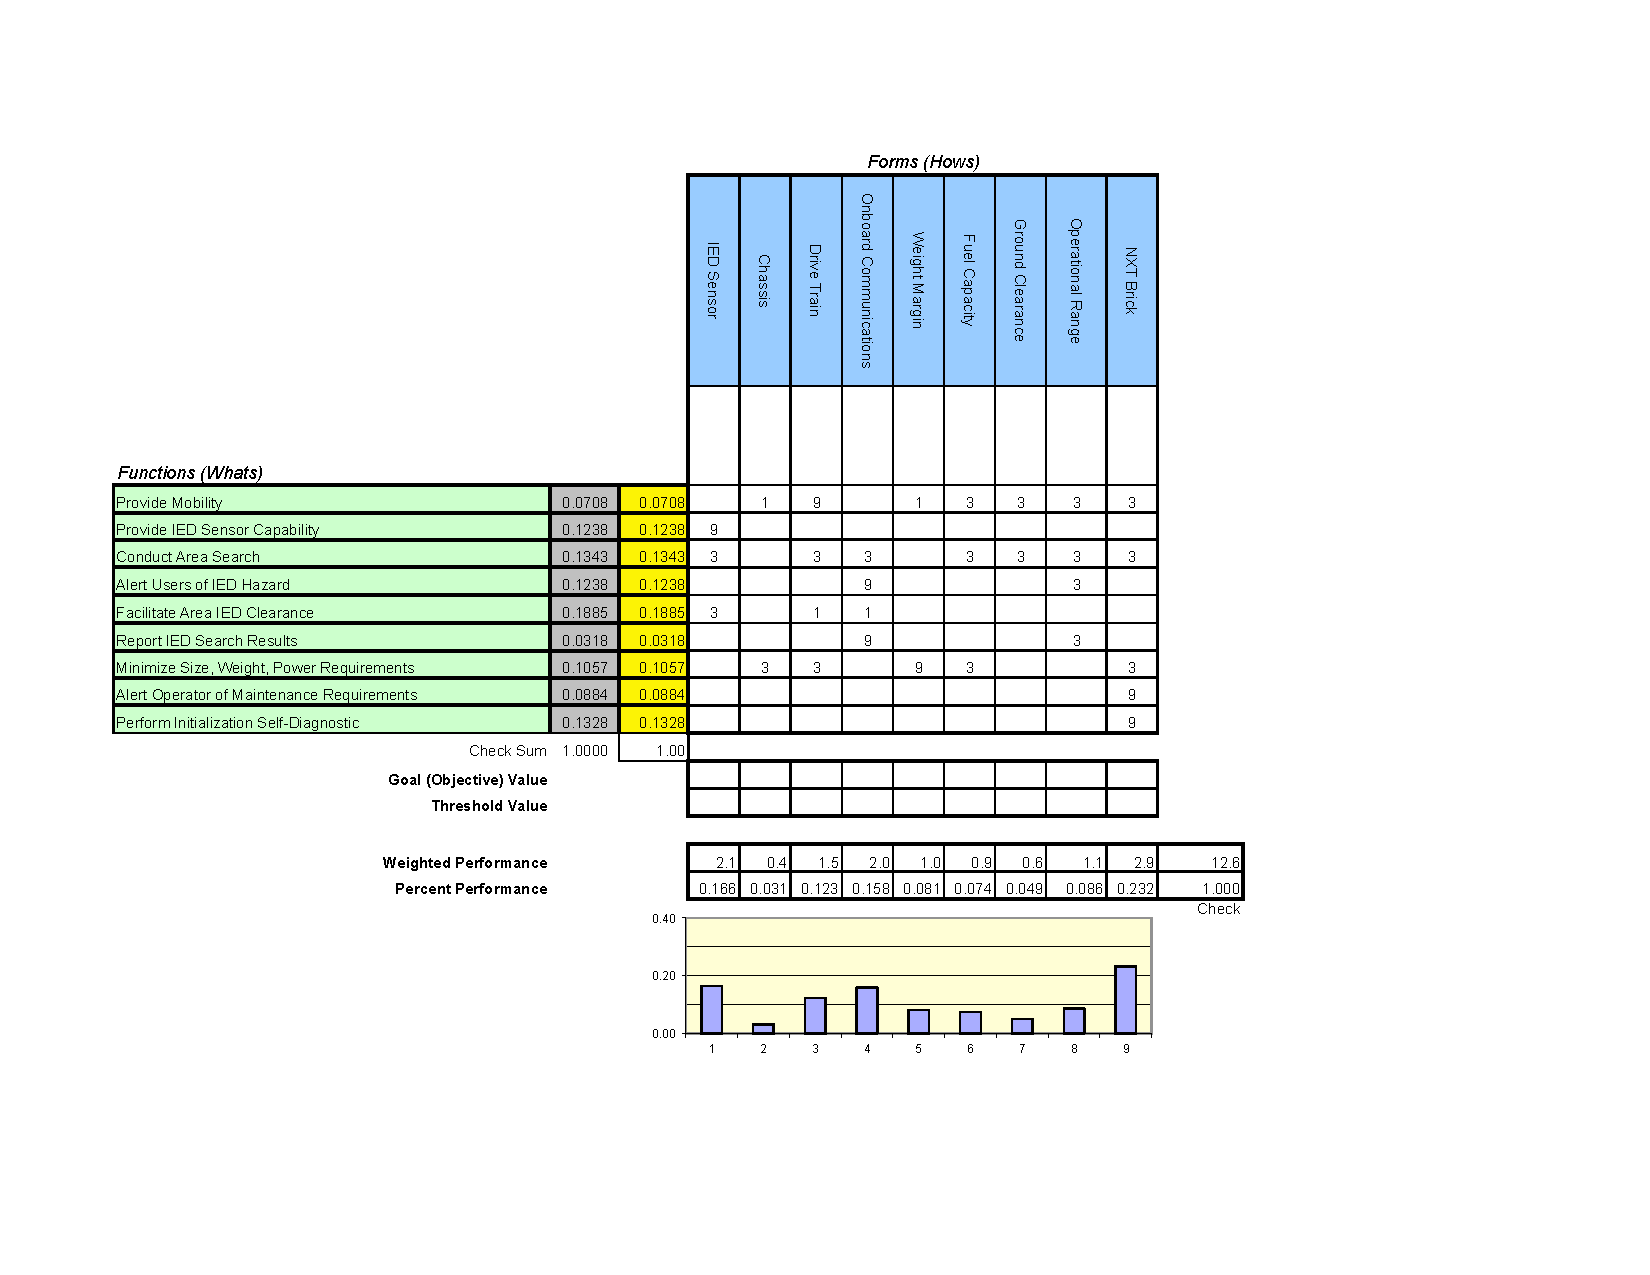
\includegraphics[scale=0.75]{QFD3b.pdf}
\caption{QFD 3 - Iraq}
\label{figQFD3b}
\end{center}
\end{figure}

\pagebreak
\section{Primary Key Performance Parameters}
HIB = Higher is Better, LIB = Lower is Better

\begin{figure}[h!tbp]
\begin{center}
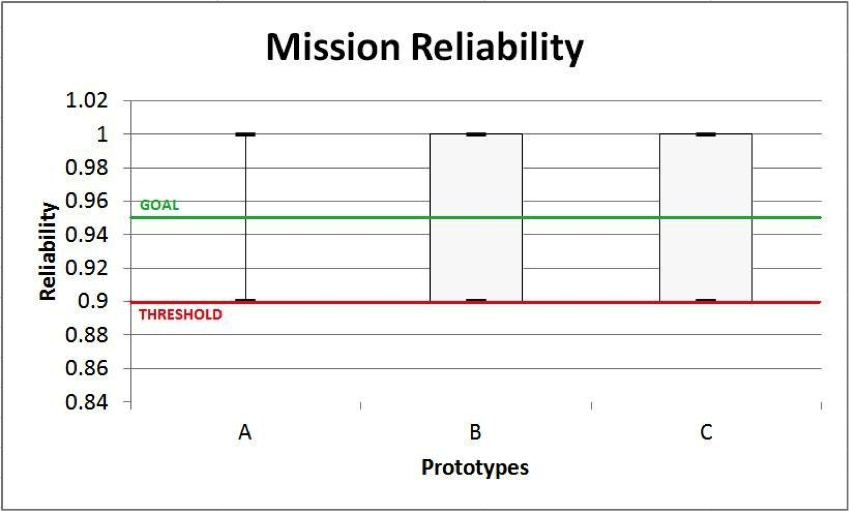
\includegraphics[scale=0.8]{missionReliability.png}
\caption{Mission Reliability}
\label{figA}
\end{center}
\end{figure}

\begin{figure}[h!tbp]
\begin{center}
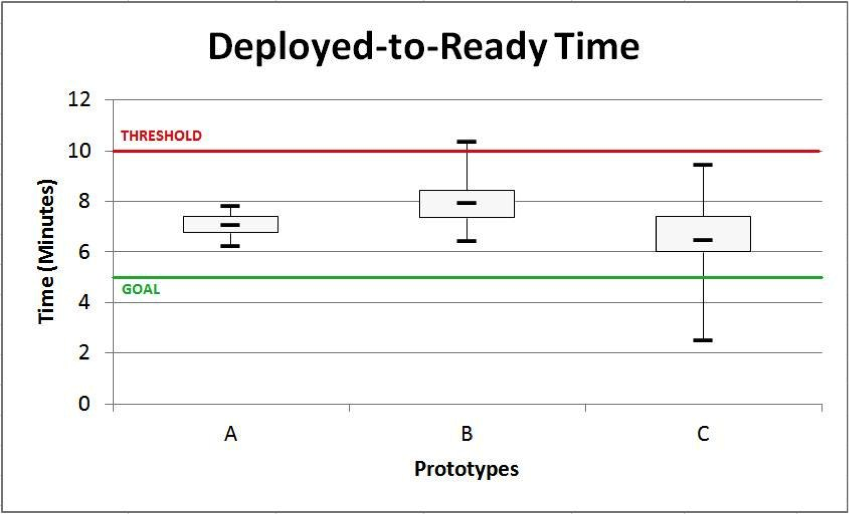
\includegraphics[scale=0.8]{deployToReadyTime.png}
\caption{Deployed-to-Ready Time}
\label{figB}
\end{center}
\end{figure}

\begin{figure}[h!tbp]
\begin{center}
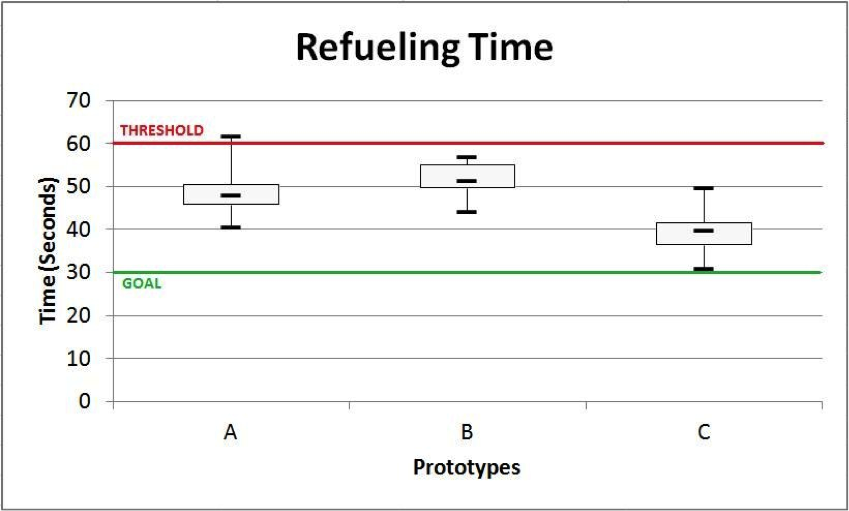
\includegraphics[scale=0.8]{refuelingTime.png}
\caption{Refueling Time}
\label{figC}
\end{center}
\end{figure}

\begin{figure}[h!tbp]
\begin{center}
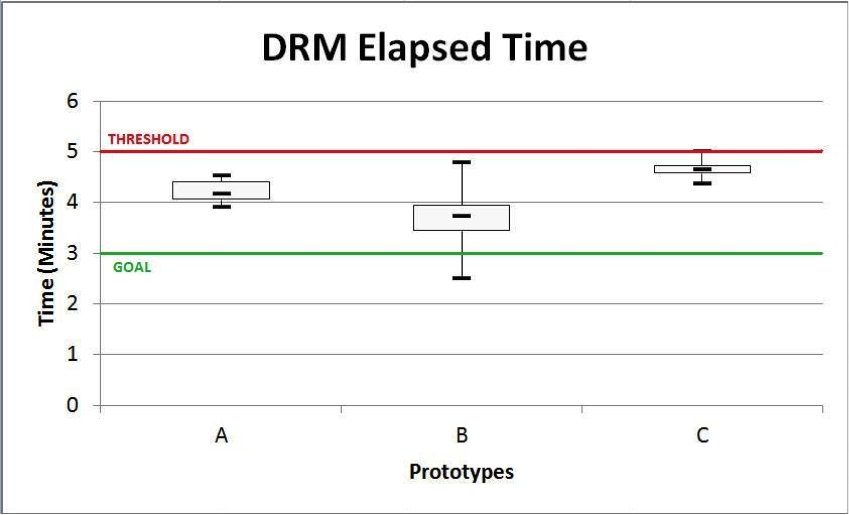
\includegraphics[scale=0.8]{drmElapsedTime.png}
\caption{DRM Elapsed Time}
\label{figD}
\end{center}
\end{figure}

\begin{figure}[h!tbp]
\begin{center}
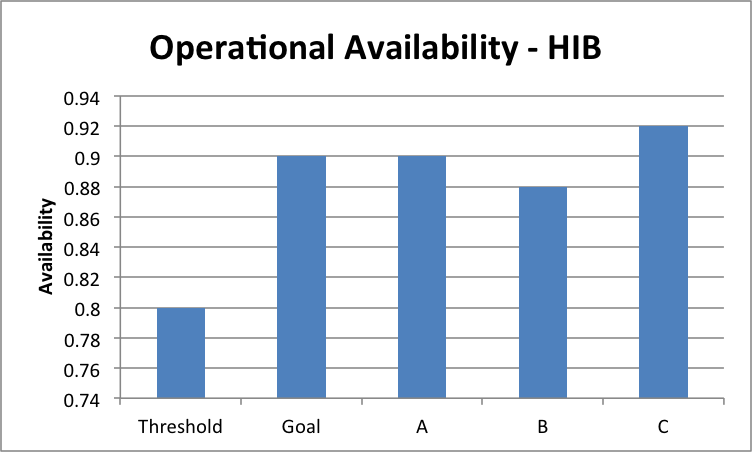
\includegraphics[scale=0.8]{operationalAvailability.png}
\caption{Operational Availability - HIB}
\label{figE}
\end{center}
\end{figure}

\begin{figure}[h!tbp]
\begin{center}
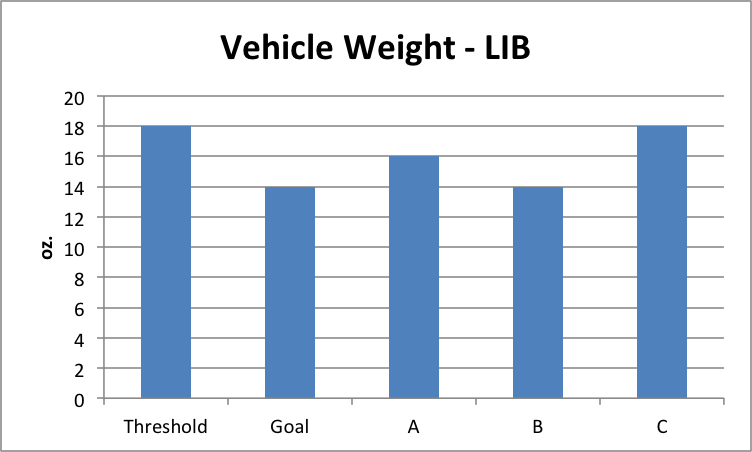
\includegraphics[scale=0.8]{vehicleWeight.png}
\caption{Vehicle Weight - LiB}
\label{figF}
\end{center}
\end{figure}

\begin{figure}[h!tbp]
\begin{center}
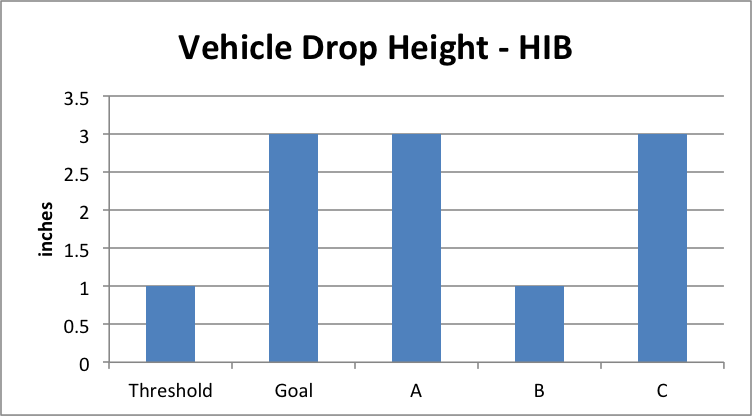
\includegraphics[scale=0.8]{vehicleDropHeight.png}
\caption{Vehicle Drop Height - HIB}
\label{figG}
\end{center}
\end{figure}

\begin{figure}[h!tbp]
\begin{center}
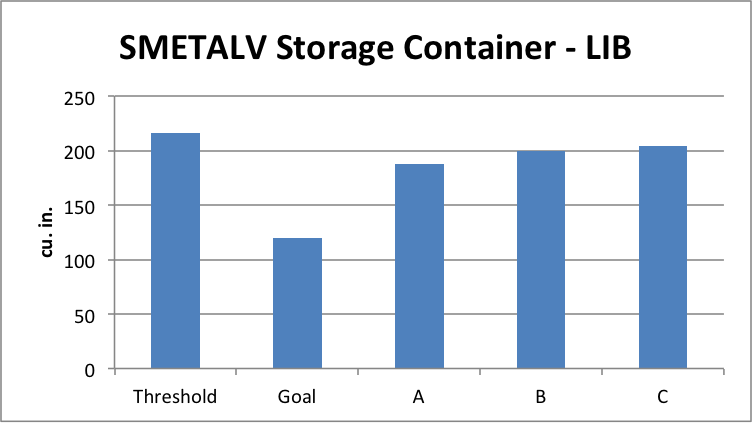
\includegraphics[scale=0.8]{storageContainer.png}
\caption{SMETALV Storage Container - LIB}
\label{figH}
\end{center}
\end{figure}

\begin{figure}[h!tbp]
\begin{center}
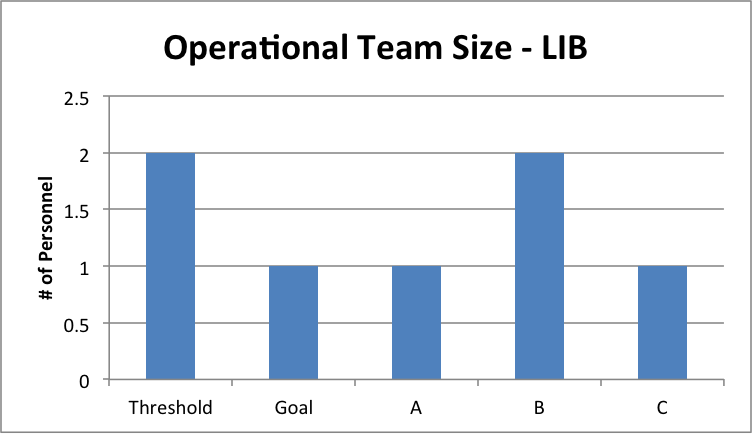
\includegraphics[scale=0.8]{operationalTeamSize.png}
\caption{Operational Team Size - LIB}
\label{figI}
\end{center}
\end{figure}

\end{document}